\section{Les disques protoplanétaire}
%TODO voir thèse mordasini, et les articles de mordasini, alibert, ida et lin, histoire de voir ce qu'ils font)


\subsection{Formation et évolution}
Les planètes se forment à partir d'un disque protoplanétaire constitué de gaz et de poussière. On observe de tels disques autour d'étoiles jeunes, essentiellement pendant les premiers millions d'années de leur existence. 

L'évolution de tels objets au cours du temps est un sujet de recherche actif, mais le principe de base est que lors de l'effondrement gravitationnel d'un nuage moléculaire diffus, le gigantesque moment angulaire de cette masse ne peut s'évacuer instantanément. 

%TODO 
\subsection{La viscosité du disque} \index{viscosité}% (Franck et al. 1992)
Quand on parle de viscosité $\nu$ dans un disque, ce n'est pas la viscosité moléculaire classique. On suppose généralement une viscosité due aux turbulences qui est beaucoup plus importante que la viscosité moléculaire, mais qui peut être traitée par les mêmes équations. 

La première hypothèse est de considérer une viscosité constante. Faute de mieux, c'est ce qui semble être le plus évident. On peut, si on veut affiner, utiliser une théorie dite des \gras{disque-alpha}

\subsubsection{Les disques alpha}
On peut introduire un paramètre adimensionné $\alpha$ \citep{shakura1989black}. Dans ce formalisme, plusieurs hypothèses sont faites : 
\begin{itemize}
\item On considère que les turbulences sont sub-soniques.
\item L'échelle des tourbillons des turbulences est plus petite que l'échelle de hauteur du disque
\end{itemize}

En conséquence, on peut définir la viscosité $\nu$ associée aux turbulences comme étant 
\begin{align}
\nu &= \alpha c_s H
\end{align}
où $c_s$ est la vitesse du son et $H$ l'échelle de hauteur du disque. $\alpha$ (avec $\alpha < 1$) est alors un paramètre adimensionné qui permet de définir plus ou moins l'intensité des turbulences, et donc la viscosité qui leur est associée. Une valeur typique d'$\alpha$ se situe entre $10^{-2}$ et $10^{-4}$.

Même si cette prescription simplifie un peu le problème, il semble probable qu'$\alpha$ ne soit pas constant, et dépende de la position dans le disque. On déplace alors le problème, vu que se pose la question des variations d'$\alpha$ dans le disque, notamment la dépendance radiale de ce dernier.

\bigskip

Le mécanisme qui a le plus de chance d'être à l'origine de la viscosité alpha est l'\gras{Instabilité Magnéto-Rotationnelle} (MRI). 

\subsection{Ionisation et dead-zones}\index{ionisation}\index{dead zone}
Pour qu'une instabilité magnéto rotationnelle ait lieu, c'est à dire qu'il y ait un couplage entre le champ magnétique et les mouvements du disque, il faut qu'une partie au moins du disque soit ionisé. Dans ces régions ionisé, on pourra alors avoir transport du moment angulaire via la viscosité due au champ magnétique (et turbulences engendrées). 

Or, comment ioniser? Que ce soit le rayonnement X de l'étoile centrale, des rayons cosmiques ou l'ionisation thermique, il n'est pas si évident que ça de se représenter l'ionisation totale du disque de gaz. Il est donc probable que certaines zones du disques ne soient pas ionisés, et donc que le transport du moment angulaire s'y fasse peu ou pas du tout. Ces zones, appelées \index{dead zone}, sont donc des zones sans viscosité magnétique. %TODO compléter la partie dead zone

\begin{figure}[htb]
\centering
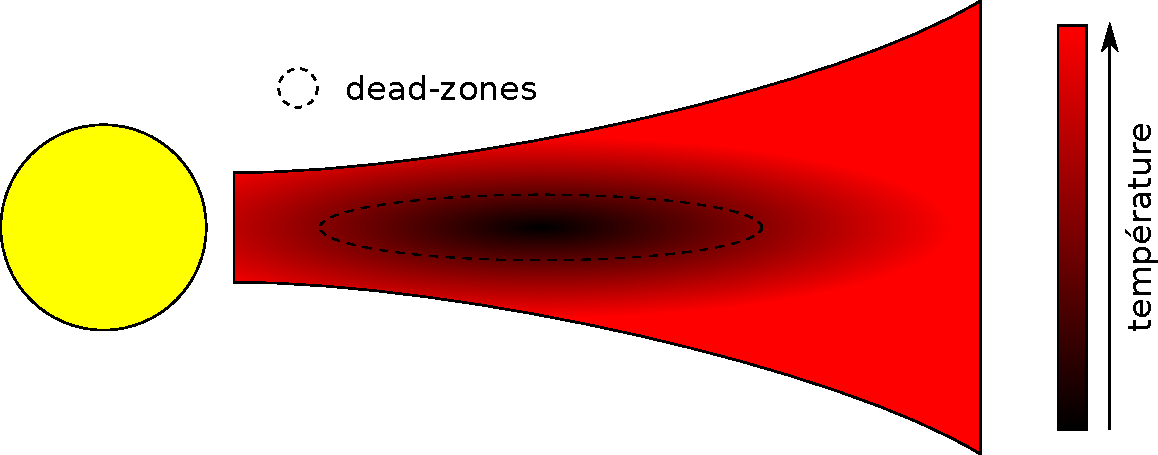
\includegraphics[width=0.7\linewidth]{figure/dead_zones.pdf}
\caption{Représentation d'un disque à couches (layered disk). L'ionisation d'une zone est déterminé par sa température. Ainsi, les zones internes à température plus faible ne sont pas ionisés et n'ont donc pas de viscosité dûes aux turbulences magnétique (MRI). Les régions externes ne sont pas des zones mortes parce qu'elles peuvent être sujettes à des ionisations non thermiques en raison de leur densité plus faible. À distance intermédiaire, le disque est trop froid pour de l'ionisation thermique, et trop dense pour de l'ionisation non thermique.}\label{fig:dead_zones}
\end{figure}


%TODO j'en suis à la page 158 du .pdf ``accretion processes in star formation''

\subsection{Profil de densité}
%TODO 
\subsection{Profil de température}
Du point de vue de la température, il y a principalement deux types de disques : 
\begin{itemize}
\item les \gras[disque actif]{disques actifs} : la source de température est le disque lui même, qui par frottements visqueux (on appelle ça le \gras{chauffage visqueux}) va émettre de la chaleur, et donc chauffer le disque ;
\item les \gras[disque passif]{disques passifs} : la source de chaleur/température est l'étoile centrale qui éclaire le disque. 
\end{itemize}

Un disque peut à la fois être actif et passif, mais généralement on essaie d'approximer, de considérer que l'un est négligeable devant l'autre. De plus, un disque aura des zones actives et des zones passives, c'est à dire que certaines zones seront principalement chauffées par la viscosité alors que d'autres le seront par l'\gras{irradiation de l'étoile}.
%TODO parler de la température du disque (et les phénomènes principaux qui ont un effet sur la température, chauffage visqueux, irradiation de l'étoile, irradiation externe. Parler dans cette partie de l'opacité, des transitions et à quoi c'est dû, des modèles had oc pour l'opacité et des incertitudes qui en découlent

\subsection{Les bords du disque}
%TODO parler des bords du disque et de tous les problèmes que ça pose

\section{Interaction disque-planète}
\subsection{Migration planétaire}
%TODO 
\subsubsection{Type I}\index{migration!type I}
Ce type de migration ne concerne que les planètes de faible masse (de l'ordre de $10M_{\oplus}$)pour lesquelles l'interaction de marée entre la planète et le disque a une réponse linéaire (Le profil de densité surfacique reste quasiment le même). Ces planètes, qui ne creusent pas de sillon (gap) dans le disque de gaz, vont migrer vers l'intérieur.

\begin{remarque}
Pour plus de détails, se référer au chapitre 9, page 188--191 de \cite{barnes2010formation} ou \cite{ward1997protoplanet} pour l'article original.
\end{remarque}

La présence d'une planète dans un disque de gaz entraine la création d'ondes de densités aux \gras[résonnance!de Lindblad]{résonances de Lindblad} \citep{goldreich1979excitation}. Le couplage gravitationnel entre les ondes de densité et la planète qui les crées abouti à un \gras{couple} qui agit sur la planète.

Lors de la création d'ondes de densité par une planète dans un disque, il se forme un déséquilibre naturel entre les couples agissant sur les disques internes et externes. La position des résonances de Lindblad externes tend à être plus proche de la planète que ne l'est celle des résonances internes.


%TODO 
\subsubsection{Type II}\index{migration!type II}
Quand une planète dans un disque devient suffisamment massive, la réponse du disque n'est plus linéaire, et des ondes de densité induites par la planète forment des chocs non loin de là où elles sont émises. La répulsion entre le disque et la planète devient si forte qu'une cavité annulaire se forme autour de l'orbite de la planète, creusant le disque de gaz.

Une fois que la cavité est formée, la planète est dite en migration de \emph{type II} : son orbite agit alors essentiellement comme une barrière entre les deux parties du disque de gaz, \emph{interne} et \emph{externe}. Du gaz peut parfois sauter le gap, ou être accrêté par la planète mais cette dernière voit son mouvement régit par le disque de gaz, se retrouvant entraînée par la migration de celui-ci.

Compte tenu que la planète a une masse de l'ordre de\footnote{Quand la masse de la planète devient supérieure à la masse du disque local, l'inertie de celle-ci devient importante afin de déterminer son taux de migration} la masse du disque local (avec lequel elle interagit), la migration se passe sur des temps de l'ordre du \gras{temps visqueux} du disque.

\begin{remarque}
Pour plus de détails, se référer au chapitre 9, page 191--192 de \cite{barnes2010formation} ou \cite{lin1986tidal} pour des détails sur les planètes capables de former un sillon dans le disque de gaz.
\end{remarque}
%TODO 
\subsubsection{Type III}\index{migration!type III}

%TODO faire ya page 192 du bouquin de barnes un truc sur \c ca, même si c'est pas explicite dans le titre.

\begin{remarque}
Pour plus de détails, se référer au chapitre 9, page 192--193 de \cite{barnes2010formation} ou \cite{masset2003runaway}.
\end{remarque}
%TODO 

\subsection{L'amortissement de l'excentricité}%circularisation
%TODO parler des autres phénomènes importants dans le disque, comme l'amortissement de l'excentricité

\subsection{L'amortissement de l'inclinaison}%coplanarisation
%TODO parler de l'amortissement de l'inclinaison, 

\subsection{L'accrétion du gaz}\label{sec:accretion_coeur}
Dans le modèle d'\gras[modèle!accrétion de c\oe ur]{accrétion de c\oe ur}, les planètes géantes sont d'abord des c\oe urs rocheux qui grossissent jusqu'à atteindre une masse critique de l'ordre de $15 M_{\oplus}$. Une fois cette masse atteinte, le c\oe ur commence à accréter rapidement du gaz jusqu'à former une géante gazeuse.

Ceci implique que la formation des planètes géantes doive se passer avant que le disque de gaz ne se dissipe (ce qui intervient au bout de $10^7$ ans environ).

Les noyaux de ces planètes sont supposés se former au delà de la ligne des glaces (limite radiale virtuelle au delà de laquelle on peut trouver de l'eau sous forme solide ; autour de $4\unit{ua}$). En effet, au delà de cette limite, la quantité de matière solide augmente, et donc le taux d'accrétion augmente aussi.

\begin{attention}
La formation des embryons de planètes géantes n'est toujours pas clair. On ne sait pas vraiment s'il y a une zone privilégiée ou non, la limite virtuelle de la ligne des glaces pourrait ne pas être valable, la glace ne rajoutant qu'environ 50\% de masse en plus.\index{ligne des glaces}\index{snowline|see{ligne des glaces}}

À noter qu'il n'y a pas de pression et donc pas de liquide dans l'espace, juste du gaz ou du solide.
\end{attention}

\bigskip

Pour une simulation donnée, si on augmente le taux d'accrétion de la planète, celle-ci sera plus massive, et aura donc une inertie plus grande. Elle mettra donc plus de temps à migrer\index{migration} par migration Type II car son inertie s'y opposera. D'un autre coté, si la planète n'a pas encore créé de gap, la migration de Type I est plus rapide à mesure que la masse augmente. 

%TODO parler de l'accrétion, et du fait que ça va créer des planètes géantes notamment

\subsection{Récapitulatif des interactions dans le code N-corps}
%TODO parler du fait que je ne prend pas en compte l'accrétion de gaz, les gaps, 